\documentclass{article}
\usepackage{graphicx}
\usepackage[utf8]{inputenc}
\usepackage{listings}
\usepackage{color}
\usepackage{xcolor}
\usepackage{textcomp}

\definecolor{solarized@base03}{HTML}{002B36}
\definecolor{solarized@base02}{HTML}{073642}
\definecolor{solarized@base01}{HTML}{586e75}
\definecolor{solarized@base00}{HTML}{657b83}
\definecolor{solarized@base0}{HTML}{839496}
\definecolor{solarized@base1}{HTML}{93a1a1}
\definecolor{solarized@base2}{HTML}{EEE8D5}
\definecolor{solarized@base3}{HTML}{FDF6E3}
\definecolor{solarized@yellow}{HTML}{B58900}
\definecolor{solarized@orange}{HTML}{CB4B16}
\definecolor{solarized@red}{HTML}{DC322F}
\definecolor{solarized@magenta}{HTML}{D33682}
\definecolor{solarized@violet}{HTML}{6C71C4}
\definecolor{solarized@blue}{HTML}{268BD2}
\definecolor{solarized@cyan}{HTML}{2AA198}
\definecolor{solarized@green}{HTML}{859900}

\lstset{
  language=Python,
  upquote=true,
  columns=fixed,
  tabsize=2,
  extendedchars=true,
  breaklines=true,
  frame=single,
  numbers=left,
  numbersep=5pt,
  rulesepcolor=\color{solarized@base03},
  numberstyle=\tiny\color{solarized@base01},
  basicstyle=\footnotesize\ttfamily,
  keywordstyle=\color{solarized@green},
  stringstyle=\color{solarized@cyan}\ttfamily,
  identifierstyle=\color{solarized@blue},
  commentstyle=\color{solarized@base01},
  emphstyle=\color{solarized@red}
}
\begin{document}

\title{Tarea 1}
\author{Angel Caceres Licona}

\maketitle


\section{Encontrar los ceros del polinomio}
Empezamos por graficar el polinomio:
\begin{center}
    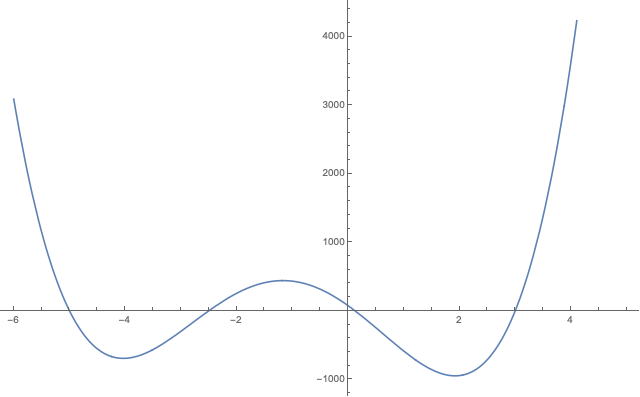
\includegraphics[scale=0.5]{grafica1.png}    
\end{center}

Para el primer punto usamos $p_0 = -8 + 0i$, $p_1 = -7 + 0i$ y $p_2 = -6 + 0i$ y obtenemos lo siguiente:

\begin{center}
    \begin{tabular}{||c c c||} 
    \hline
    $n$ & $p_{n}$ & $f(p_n)$ \\ [0.5ex] 
    \hline
    0 & -5.56988770741102+0j & 1366.1300931573928+0j\\
    \hline
    1 & -5.253213136295214+0j & 495.11617890693424+0j \\
    \hline
    2 & -5.098845924131111+0j & 173.8892671646845+0j \\
    \hline
    3 & -5.024791372074857+0j & 41.38752244099669+0j \\ 
    \hline
    4 & -5.003476678249181+0j & 5.716037928335936+0j \\ 
    \hline
    5 & -5.000158597502512+0j & 0.26012961100877874+0j \\ 
    \hline
    6 & -5.000001181494323+0j & 0.0019376523382561572+0j \\ 
    \hline
    7 & -5.000000000421358+0j & 6.910286174388602e-07+0j \\ 
    \hline
    8 & -5+0j & 0j \\ [1ex]
    \hline
   \end{tabular}
\end{center}


Para el segundo punto usamos $p_0 = -5.5 + 0i$, $p_1 = -4+0i$ y $p_2 = -3+0i$ y obtenemos lo siguiente:
\begin{center}
    \begin{tabular}{||c c c||} 
    \hline
    $n$ & $p_{n}$ & $f(p_n)$ \\ [0.5ex] 
    \hline
    0 & -2.73014360107805+0j & -136.74477205133985+0j\\
    \hline
    1 & -2.5499814337627+0j & -29.08776618373531+0j \\
    \hline
    2 & -2.507713928583022+0j &-4.460345829948892+0j \\
    \hline
    3 & -2.5003258053984068+0j & -0.18816259248796996+0j \\ 
    \hline
    4 & -2.500002511682252+0j & -0.0014504970934012817+0j \\ 
    \hline
    5 & -2.5000000008553442+0j & -4.939613518217811e-07+0j \\ 
    \hline
    6 & -2.500000000000002+0j & -1.3642420526593924e-12+0j \\ [1ex]
    \hline

   \end{tabular}
\end{center}

Para el tercer punto usamos $p_0 = -1 + 0i$, $p_1 = -0.5 + 0i$ y $p_2 = -0 + 0i$ y obtenemos lo siguiente:
\begin{center}
    \begin{tabular}{||c c c||} 
    \hline
    $n$ & $p_{n}$ & $f(p_n)$ \\ [0.5ex] 
    \hline
    0 & 0.10636615495378643+0j & 11.48189096004183+0j\\
    \hline
    1 & 0.12432985679642755+0j & 0.4146504754316993+0j \\
    \hline
    2 & 0.12499576897414577+0j & 0.0026183413773708253+0j \\
    \hline
    3 & 0.12499999900157793+0j& 6.178672578016631e-07+0j \\ 
    \hline
    4 & 0.1249999999999985+0j & 9.237055564881302e-13+0j \\ [1ex]
    \hline

   \end{tabular}
\end{center}

Para el cuarto punto usamos $p_0 = 1 + 0i$, $p_1 = 1.5 + 0i$ y $p_2 = 2 + 0i$ y obtenemos lo siguiente:
\begin{center}
    \begin{tabular}{||c c c||} 
    \hline
    $n$ & $p_{n}$ & $f(p_n)$ \\ [0.5ex] 
    \hline
    0 & 0.10636615495378643+0j & 11.48189096004183+0j\\
    \hline
    1 & 0.12432985679642755+0j & 0.4146504754316993+0j \\
    \hline
    2 & 0.12499576897414577+0j & 0.0026183413773708253+0j \\
    \hline
    3 & 0.12499999900157793+0j& 6.178672578016631e-07+0j \\ 
    \hline
    4 & 0.1249999999999985+0j & 9.237055564881302e-13+0j \\ [1ex]
    \hline

   \end{tabular}
\end{center}


\section{2o ejercicio}
Encontrar las raíces del polinomio $x^5 -3.4x^4 + 5.4521x^3 -4.2077x^2 + 1.50924x - 0.20304$

Empezamos por graficar el polinomio para localizar las raíces:
\begin{center}
    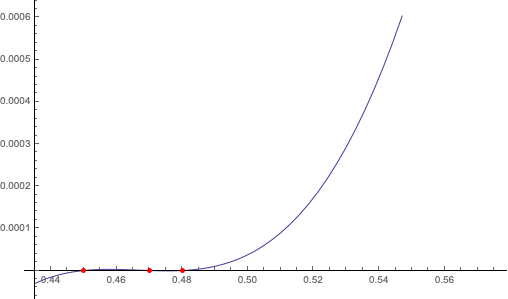
\includegraphics[scale=0.5]{grafica2.png}    
\end{center}

Para el primer punto usamos $p_0 = 0.1 + 0i$, $p_1 = 0.2 + 0i$ y $p_2 = 0.3 + 0i$ y obtenemos lo siguiente:

\begin{center}
    \begin{tabular}{||c c c||} 
    \hline
    $n$ & $p_{n}$ & $f(p_n)$ \\ [0.5ex] 
    \hline
    0 & 0.4458286112629127+0j & -4.5035571730744905e-06+0j\\
    \hline
    1 & 0.447862249714668+0j & -1.984579714342516e-06+0j \\
    \hline
    2 & 0.44911066631197444+0j & -7.480005712046101e-07+0j \\
    \hline
    3 & 0.44973410889903526+0j & 0.44973410889903526+0j \\ 
    \hline
    4 & 0.4499539551055597+0j & -3.612369059435849e-08+0j \\ 
    \hline
    5 & 0.44999683279627883+0j & -2.4758296524041157e-09+0j \\ 
    \hline
    6 & 0.44999995472396714+0j & -3.5383473928618514e-11+0j \\ 
    \hline
    7 & 0.4499999999522736+0j & -3.735900477863652e-14+0j \\ 
    \hline
    8 & 0.450000000000077+0j & 0j \\ [1ex]
    \hline
   \end{tabular}
\end{center}

Para el segundo punto usamos $p_0 = 0.44449 + 0i$, $p_1 = 0.45 + 0i$ y $p_2 = 0.46 + 0i$ y obtenemos lo siguiente:

\begin{center}
    \begin{tabular}{||c c c||} 
    \hline
    $n$ & $p_{n}$ & $f(p_n)$ \\ [0.5ex] 
    \hline
    0 & 0.46361984035922454-0.006480490395900713j & 2.315981070533102e-06+2.077710561383672e-06j\\
    \hline
    1 & 0.4644536016521566-0.0013817275971592683j& 1.6195876901825557e-06+3.940042875242439e-07j \\
    \hline
    2 & 0.4681675684182604-0.0016224161844768433j & 4.894803319333008e-07+4.777100273906446e-07j \\
    \hline
    3 & 0.46941074191987503-0.0005016559512962782j & 1.5250603035976695e-07+1.357088822529851e-07j \\ 
    \hline
    4 & 0.46996400037246505-0.0001786353845617478j & 8.828068498445418e-09+4.5936642648156806e-08j \\ 
    \hline
    5 & 0.4700099838395804-1.818521082275532e-05j & -2.5606796683064204e-09+4.653959900532918e-09j \\ 
    \hline
    6 & 0.47000065692413423+3.1214107531578656e-07j & -1.682864958496566e-10-7.995896020945756e-11j \\ 
    \hline
    7 & 0.46999999705608536+1.2287968008216802e-09j & 7.541745006278688e-13-3.147932586412226e-13j \\ 
    \hline
    8 & 0.470000000000476+1.5254619116459673e-13j & -2.220446049250313e-16-3.907928325070722e-17j \\ [1ex]
    \hline
   \end{tabular}
\end{center}

Para el tercer punto usamos $p_0 = 0.46 + 0i$, $p_1 = 0.47002 + 0i$ y $p_2 = 0.48321 + 0i$ y obtenemos lo siguiente:

\begin{center}
    \begin{tabular}{||c c c||} 
    \hline
    $n$ & $p_{n}$ & $f(p_n)$ \\ [0.5ex] 
    \hline
    0 & 0.47660443303598554+0j & -7.600668973095637e-07+0j\\
    \hline
    1 & 0.47989521248348477+0j & -3.938347747922677e-08+0j \\
    \hline
    2 & 0.47999870157997+0j & -4.947687815004542e-10+0j \\
    \hline
    3 & 0.4800000011944164+0j & 4.551914400963142e-13+0j \\ 
    \hline
    4 & 0.48000000000005055+0j & -1.1102230246251565e-16+0j \\ [1ex]
    \hline
   \end{tabular}
\end{center}

Para el cuarto punto usamos $p_0 = 0.96 - 0.96i$, $p_1 = 0.97 - 0.97i$ y $p_2 = 0.98 - 0.98i$ y obtenemos lo siguiente:

\begin{center}
    \begin{tabular}{||c c c||} 
    \hline
    $n$ & $p_{n}$ & $f(p_n)$ \\ [0.5ex] 
    \hline
    0 & 0.999999989509428-0.9999999819177748j & -5.54634412841537e-08-2.507695140430144e-08j\\
    \hline
    1 & 1.0000000153197894-0.9999999870935946j& -3.288684002900055e-08+4.8170878397257866e-08j\\
    \hline
    2 & 1.0000000147687256-1.000000005888029j & 2.139572685688762e-08+4.105273565535583e-08j \\
    \hline
    3 & 1.0000000006269771-1.0000000024209634j & 7.197350604393193e-09+1.104973446075519e-09j \\ 
    \hline
    4 & 1.0000000016368629-0.9999999988980542j& -2.7112517786420653e-09+5.065483144051086e-09j \\ [1ex]
    \hline
   \end{tabular}
\end{center}


Para el cuarto punto usamos $p_0 = 0.96 + 0.96i$, $p_1 = 0.97 + 0.97i$ y $p_2 = 0.98 + 0.98i$ y obtenemos lo siguiente:

\begin{center}
    \begin{tabular}{||c c c||} 
    \hline
    $n$ & $p_{n}$ & $f(p_n)$ \\ [0.5ex] 
    \hline
    0 & 0.999999989509428+0.9999999819177748j & -5.54634412841537e-08+2.507695140430144e-08j\\
    \hline
    1 & 1.0000000153197894+0.9999999870935946j & -3.288684002900055e-08-4.8170878397257866e-08j\\
    \hline
    2 & 1.0000000147687256+1.000000005888029j & 2.139572685688762e-08-4.105273565535583e-08j \\
    \hline
    3 & 1.0000000006269771+1.0000000024209634j & 7.197350604393193e-09-1.104973446075519e-09j \\ 
    \hline
    4 & 1.0000000016368629+0.9999999988980542j & -2.7112517786420653e-09-5.065483144051086e-09j \\ [1ex]
    \hline
   \end{tabular}
\end{center}


\section{3er ejercicio}
Encontrar las raíces del polinomio $4x^4 -9x^3 + 3x^2 +5x -3$

Empezamos por graficar el polinomio para localizar las raíces:
\begin{center}
    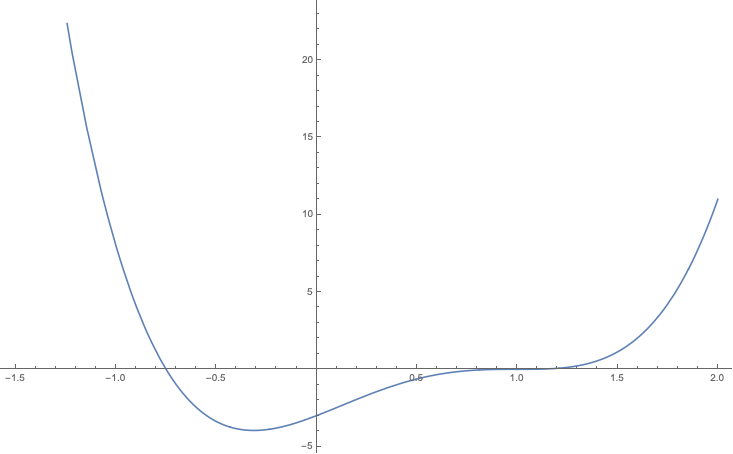
\includegraphics[scale=0.5]{grafica3.png}    
\end{center}

Para el primer punto usamos $p_0 = -1.2 + 0i$, $p_1 = -1 + 0i$ y $p_2 = -0.7 + 0i$ y obtenemos lo siguiente:

\begin{center}
    \begin{tabular}{||c c c||} 
    \hline
    $n$ & $p_{n}$ & $f(p_n)$ \\ [0.5ex] 
    \hline
    0 & -0.7496075804729001+0.00014754164740447048j & -0.008407635090922128-0.0031586699106211555j\\
    \hline
    1 & -0.7499936143696264+3.4158211366882337e-06j & -0.00013689088140012018-7.322506243110868e-05j\\
    \hline
    2 & -0.7499999895530871-3.1236003243294187e-09j & -2.239556913252727e-07+6.696217955436136e-08j \\
    \hline
    3 & -0.7499999999998296-2.325816020044391e-13j & -3.652633751016765e-12+4.98596809296725e-12j \\ 
    \hline
    4 & -0.75-8.415717376759247e-21j & 1.8041194126427636e-19j \\ [1ex]
    \hline
   \end{tabular}
\end{center}

Para el segundo punto usamos $p_0 = 0.7 + 0i$, $p_1 = 0.8 + 0i$ y $p_2 = 0.9 + 0i$ y obtenemos lo siguiente:

\begin{center}
    \begin{tabular}{||c c c||} 
    \hline
    $n$ & $p_{n}$ & $f(p_n)$ \\ [0.5ex] 
    \hline
    0 & 0.9999917539097252+0j & -3.9968028886505635e-15+0j\\
    \hline
    1 & 0.9999930288112501+0j & -2.6645352591003757e-15+0j\\
    \hline
    2 & 0.9999949014295727+0j & -2.239556913252727e-07+6.696217955436136e-08j \\
    \hline
    3 & 0.9999969129400132+0j & 0j \\ [1ex]
    \hline
   \end{tabular}
\end{center}

\section{4o ejercicio}
Encuentre la raíz en el intervelo $(1,4)$ de la ecuación $0=tan(x) -x$...
Graficamos la ecuación:
\begin{center}
    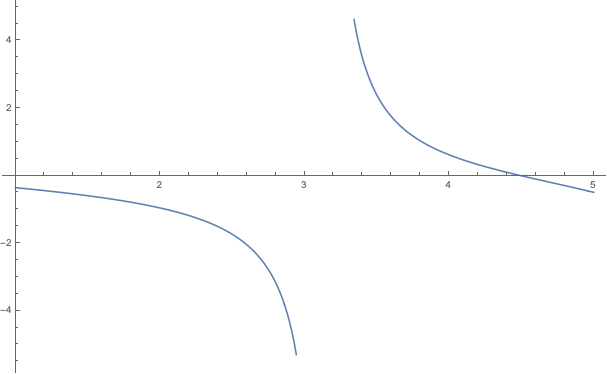
\includegraphics[scale=0.5]{graficaTan.png}    
\end{center}
Obtuve la siguiente salida: 
\begin{center}
    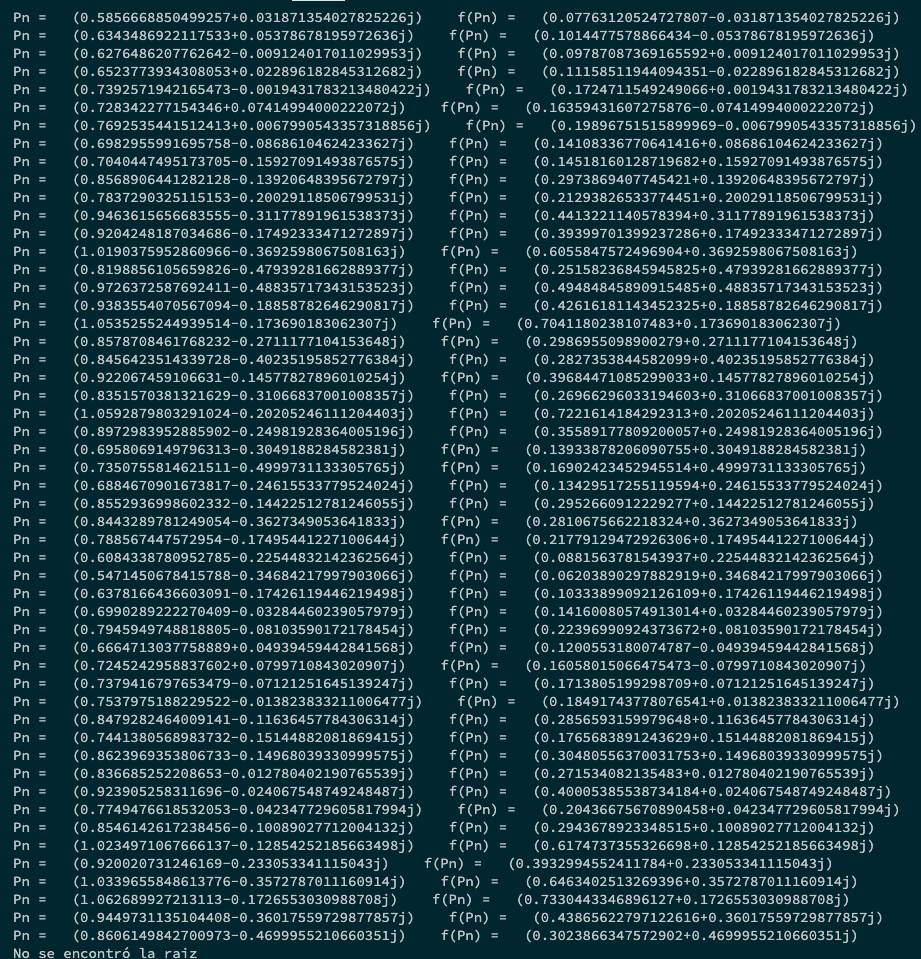
\includegraphics[scale=0.3]{salidaMuller1.png}    
\end{center}
como podemos ve el metodo no converge.
Usando la otra forma de la ecuación obtuve lo siguiente:

\begin{center}
    \begin{tabular}{||c c c||} 
    \hline
    $n$ & $p_{n}$ & $f(p_n)$ \\ [0.5ex] 
    \hline
    0 & 4.49331814720452 & 9.13125603730081e-5 \\
    \hline
    1 & 4.49340765899325 & 1.79891653645514e-6\\
    \hline
    2 & 4.49340945620222 & 1.70684263944842e-9 \\
    \hline
    3 & 4.49340945790903 & 3.2834845953289e-14 \\ [1ex]
    \hline
   \end{tabular}
\end{center}

Y como podemos observar me dio una raiz fuera del intervalo aunque en la gradica vemos que efectivamente la raiz está fuera del intervalo dado.

\section{5o ejercicio}
Encontrar las raíces complejas cercanas al origen de la ecuación $x - \sin(x)$

Empezamos por graficar el polinomio para localizar las raíces:
\begin{center}
    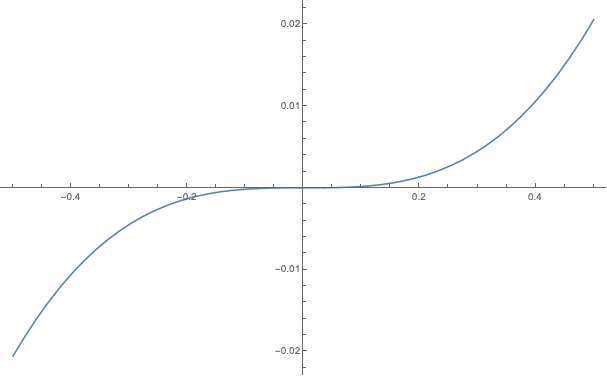
\includegraphics[scale=0.5]{graficaSin.png}    
\end{center}

Esta función sólo tiene una raiz real en $(0,0)$

Usando los puntos $p_0 = -0.1 + 0i$, $p_1 =0.001 + 0i$ y $p_2 = 0.00001 + 0i$ obtuve

\begin{center}
    \begin{tabular}{||c c c||} 
    \hline
    $n$ & $p_{n}$ & $f(p_n)$ \\ [0.5ex] 
    0 & 0.001000903020366235  & 1.6711857635590133e-10 \\ [1ex]
    \hline
   \end{tabular}
\end{center}


\section{Codigo del programa}

\begin{lstlisting}
    def MullerM(f,p0,p1,p2,tol,maxIter):
    from numpy.lib.scimath import sqrt
    p0 = p0
    p1 = p1
    p2 = p2
    f0 = f(p0)
    f1 = f(p1)
    f2 = f(p2)
    f3 = 0
    i = 0
    while i<=maxIter:
        c = f2
        b = ((p0-p2)**2 *(f1-f2)-(p1-p2)**2 *(f0-f2))/((p0-p2)*(p1-p2)*(p0-p1))
        a = ((p1-p1)*(f0-f2) - (p0-p2)*(f1-f2))/((p0-p2)*(p1-p2)*(p0-p1))
        p3 = p2 - 2*c/(b+(b/abs(b))*sqrt(b**2 -4*a*c))
        f3 = f(p3)
        print ("Pn =  ", p3, "   f(Pn) =  ", f3)
        if abs(p3-p2)<tol:
            return p3
        p0 = p1
        p1 = p2
        p2 = p3
        f0 = f(p0)
        f1 = f(p1)
        f2 = f(p2)
        i = i+1
    print ("No se encontro la raiz")
    
def f(x):
    fx = 16*x**4 + 70*x**3 -169*x**2 -580*x + 75
    return fx

MullerM(f,complex(1.5,0),complex(2,0),complex(2.5,0),0.00000001,100)
\end{lstlisting}


\end{document}